Till now we treated the simplest model, where at the moment of spawning the cAMP was a lonely molecule simply roaming around of \Bm.
This is though very far from reality, where the cAMP is released in waves expanding radially around the amoeba.


[[here quote some paper AND some youtube video connected to it]]

Let us then fix the spatial dimension $d=2$ for the sake of simplicity, and consider always the same Poisson process $(\hmactive_t^p)_p$.
Let $\NumCampRelease \in \N$ be the (deterministic) number of cAMP molecules being spawned at each birth time $\btime^{p,g}$ and let $\cdrift \in \R_+$ be the (constant deterministic) modulus of their drift velocity at each of these instants.
Then, at each $\btime^{p,g}=\btime_m$ we would release the particles

\begin{equation*}
	\{ \camp^{p,g,1}, \ldots, \camp^{p,g,l}, \camp^{p,g,\NumCampRelease}\} = \{ \camp^{m,1}, \ldots, \camp^{m,l}, \camp^{m,\NumCampRelease}\} 
\end{equation*}

While the dynamic equation for the $N$ amoebas remains the same, at this point the dynamic for the cAMP changes.
First, each of them will have its quasi-\Bm.
Besides that, we can imagine this molecules to spawn at random directions







\begin{center}
	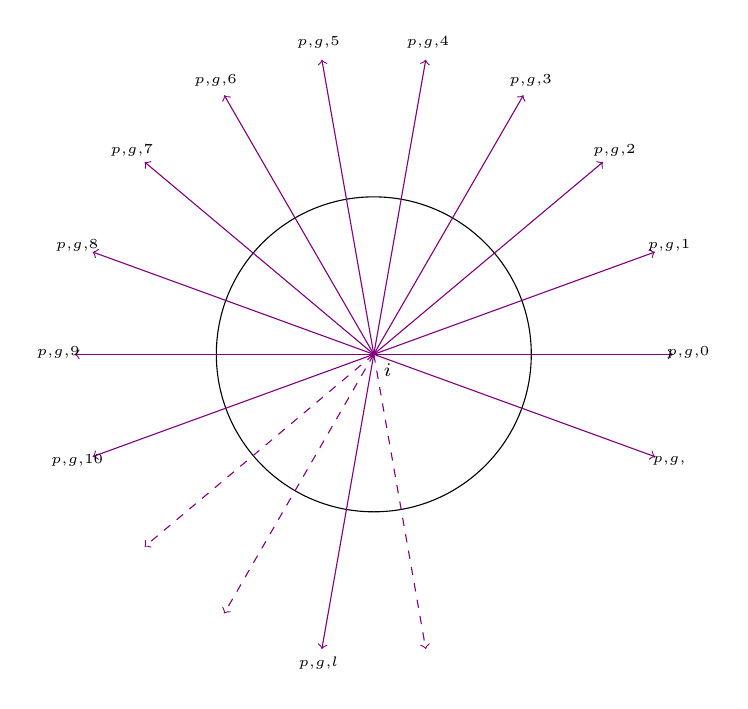
\begin{tikzpicture}
		\coordinate (center) at (0,0);
		
		\draw[thin] (center) circle (2cm);
		
		\foreach \index in {0,1,...,12} {
			\coordinate (A) at (canvas polar cs:radius=3.8cm,angle=20*\index);
			
			\ifnum \index < 11
			\draw[violet,->] (center) -- (A);
			\coordinate (B) at (canvas polar cs:radius=4cm,angle=20*\index);
			\node at (B) {\tiny $\camp^{p,g,\index}$};
			\else
			\draw[violet,dashed,->] (center) -- (A);
			\fi
		}
		
		\coordinate (A) at (canvas polar cs:radius=3.8cm,angle=20*13);
		\draw[violet,->] (center) -- (A);
		
		\coordinate (B) at (canvas polar cs:radius=4cm,angle=20*13);
		\node at (B) {\tiny $\camp^{p,g,l}$};
		
		\coordinate (A) at (canvas polar cs:radius=3.8cm,angle=20*14);
		\draw[violet,dashed,->] (center) -- (A);
		
		\coordinate (A) at (canvas polar cs:radius=3.8cm,angle=340);
		\draw[violet,->] (center) -- (A);
		
		\coordinate (B) at (canvas polar cs:radius=4cm,angle=340);
		\node at (B) {\tiny $\camp^{p,g,\NumCampRelease}$};
		
		\node[anchor=north west] at (center) {$\amba^i$};
	\end{tikzpicture}
\end{center}